%%%%%%%%%%%%%%%%%%%%%%%%%%%%%%%%%%%%%%%%%%%%%%%%%%%%%%%%%%%%%%%%%
% MUW Presentation
% LaTeX Template
% Version 1.0 (27/12/2016)
%
% License:
% CC BY-NC-SA 4.0 (http://creativecommons.org/licenses/by-nc-sa/3.0/)
%
% Created by:
% Nicolas Ballarini, CeMSIIS, Medical University of Vienna
% nicoballarini@gmail.com
% http://statistics.msi.meduniwien.ac.at/
%
% Customized for UAH by:
% David F. Barrero, Departamento de Automática, UAH
%%%%%%%%%%%%%%%%%%%%%%%%%%%%%%%%%%%%%%%%%%%%%%%%%%%%%%%%%%%%%%%%%

\documentclass[10pt,compress]{beamer} % Change 10pt to make fonts of a different size
\mode<presentation>

\usepackage[spanish]{babel}
\usepackage{fontspec}
\usepackage{tikz}
\usepackage{etoolbox}
\usepackage{xcolor}
\usepackage{xstring}
\usepackage{listings}

\usetheme{UAH}
\usecolortheme{UAH}
\setbeamertemplate{navigation symbols}{} 
\setbeamertemplate{caption}[numbered]

%%%%%%%%%%%%%%%%%%%%%%%%%%%%%%%%%%%%%%%%%%%%%%%%%%%%%%%%%%%%%%%%%
%% Presentation Info
\title[An informal introduction to Python]{An informal introduction to Python}
\author{}
\institute{\asignatura}
\date{}
%%%%%%%%%%%%%%%%%%%%%%%%%%%%%%%%%%%%%%%%%%%%%%%%%%%%%%%%%%%%%%%%%


%%%%%%%%%%%%%%%%%%%%%%%%%%%%%%%%%%%%%%%%%%%%%%%%%%%%%%%%%%%%%%%%%
%% Descomentar para habilitar barra de navegación superior
\ponerNavegacion
%%%%%%%%%%%%%%%%%%%%%%%%%%%%%%%%%%%%%%%%%%%%%%%%%%%%%%%%%%%%%%%%%

%%%%%%%%%%%%%%%%%%%%%%%%%%%%%%%%%%%%%%%%%%%%%%%%%%%%%%%%%%%%%%%%%
%% Configuración de logotipos en portada
%% Opacidad de los logotipos
\newcommand{\opacidad}{1}
%% Descomentar para habilitar logotipo en pié de página de portada
\renewcommand{\logoUno}{Images/isg.png}
%% Descomentar para habilitar logotipo en pié de página de portada
%\renewcommand{\logoDos}{Images/CCLogo.png}
%% Descomentar para habilitar logotipo en pié de página de portada
%\renewcommand{\logoTres}{Images/ALogo.png}
%% Descomentar para habilitar logotipo en pié de página de portada
%\renewcommand{\logoCuatro}{Images/ELogo.png}
%%%%%%%%%%%%%%%%%%%%%%%%%%%%%%%%%%%%%%%%%%%%%%%%%%%%%%%%%%%%%%%%%

%%%%%%%%%%%%%%%%%%%%%%%%%%%%%%%%%%%%%%%%%%%%%%%%%%%%%%%%%%%%%%%%%
%% FOOTLINE
%% Comment/Uncomment the following blocks to modify the footline
%% content in the body slides. 


%% Option A: Title and institute
\footlineA
%% Option B: Author and institute
%\footlineB
%% Option C: Title, Author and institute
%\footlineC
%%%%%%%%%%%%%%%%%%%%%%%%%%%%%%%%%%%%%%%%%%%%%%%%%%%%%%%%%%%%%%%%%

\begin{document}

%%%%%%%%%%%%%%%%%%%%%%%%%%%%%%%%%%%%%%%%%%%%%%%%%%%%%%%%%%%%%%%%%
% Use this block for a blue title slide with modified footline
{\titlepageBlue
    \setbeamertemplate{headline}{}
	\setbeamercolor{frametitle}{bg=black}
	\setbeamercolor{normal text}{bg=black}
    \begin{frame}
        \titlepage
    \end{frame}
}

\begin{frame}[plain]{}
	\begin{block}{Objectives}
		\begin{enumerate}
		\item Understand the main Python features, strengths and weaknesses
		\item Overview the main Python statements
		\item Being able to program na\"ive Python scripts
		\end{enumerate}
	\end{block}
\end{frame}

{
\eliminarNavegacion
\begin{frame}[shrink]{Table of Contents}
 \frametitle{Table of Contents}
 \tableofcontents
  % You might wish to add the option [pausesections]
\end{frame}
}

\section{Introduction}
\subsection{What is Python?}

\begin{frame}{Introduction}{What is Python?}
    \begin{columns}
 	   \column{.70\textwidth}
			Python is a general-purpose, high-level, interpreted programming language
				\begin{itemize}
				\item \textit{General-purpose}: Many applications.
				\item \textit{High-level}: Abstract data structures, doing more with less code.
				\item \textit{Interpreted}: No need to compile.
				\end{itemize}

 	   \column{.20\textwidth}
		\centering \hspace{-2cm} 
\includegraphics[width=1.8\linewidth]{figs/python.png}
	\end{columns}
	\bigskip
			It emphasizes code \textbf{readibility} and programmer's productivity\\
\end{frame}

\subsection{Features}
\begin{frame}{Introduction}{Features}
    \begin{columns}
 	   \column{.60\textwidth}
		\vspace{-0.3cm}
		\begin{itemize}
		\item Several paradigms
			\begin{itemize}
			\item OO, imperative and functional
			\end{itemize}
		\item Dynamic typing
		\item Interpreted
		\item Minimalistic syntax
		\item Portable
		\item Extensible - Bindings to other languages
		\item Embeddable
		\item Application domains
			\begin{itemize}
			\item Web, robotics, data science, game development, admin ...
			\end{itemize}
		\end{itemize}
 	   \column{.40\textwidth}
		\centering 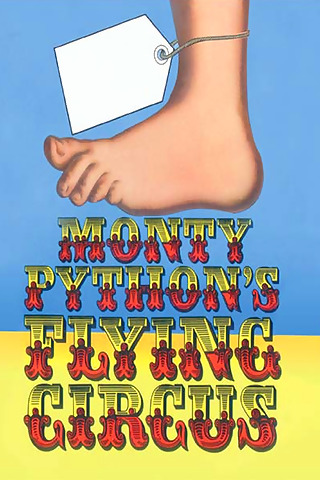
\includegraphics[width=0.9\linewidth]{figs/monty.jpg}\\
		\tiny{\href{https://www.youtube.com/watch?v=anwy2MPT5RE}{Want to know other Monty Python's contribution to Computer Science? Click here}}
	   \end{columns}
\end{frame}


\subsection{Why Python?}
\begin{frame}[plain]{Introduction}{Why Python? (I)}
		\centering 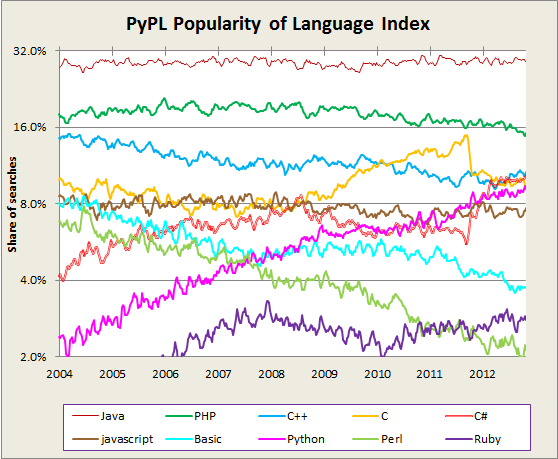
\includegraphics[width=0.8\linewidth]{figs/chart.png}\\
		\begin{center}
			\tiny{\href{http://rz.scale-it.pl/2013/01/07/python___language_of_the_decade.html}{(Source)}}
		\end{center}
\end{frame}

\begin{frame}[plain]{Introduction}{Why Python? (II)}
\centering \textit{Hello world!} examples
    \begin{columns}
 	   \column{.50\textwidth}
		\vspace{-0.2cm}
		\begin{block}{Python}
		\vspace{-0.2cm}
			\lstinputlisting{code/hello.py}
		\end{block}

		\vspace{-0.2cm}
		\begin{block}{Java}
		\vspace{-0.2cm}
			\lstinputlisting[language=java,basicstyle=\scriptsize]{code/hello.java}
		\end{block}
 	   \column{.50\textwidth}

		\vspace{-0.2cm}
		\begin{block}{C}
		\vspace{-0.2cm}
			\lstinputlisting[language=c,basicstyle=\scriptsize]{code/hello.c}
		\end{block}

		\vspace{-0.2cm}
		\begin{block}{C++}
		\vspace{-0.2cm}
			\lstinputlisting{code/hello.cpp}
		\end{block}
	\end{columns}

\end{frame}

\begin{frame}{Introduction}{Why Python? (III)}
	More reasons to love Python
	\begin{itemize}
	\item Very easy to learn ...
	\begin{itemize}
		\item ... yet extremely powerful
		\item  Clearner syntax compared to almost anything else
	\end{itemize}
	\item Facilities in development
	\begin{itemize}
	\item \small{Wide standard library: \url{http://docs.python.org/library/}}
    \item \small{Great number of modules.}
   \item \small{Almost any software library has its associated wrapping in order to its access from Python.}
		% fácil desarrollo de envolturas para manejar software en C/C++, Fortran, etc., desde python.
   \end{itemize}
	\item Interactive mode
	\begin{itemize}
		\item Rapid testing and development
	\end{itemize}
	\item Most languages are made to make big and fast programs
	\begin{itemize}
		\item Python was designed to ease programmers' life
	\end{itemize}
	\item It is free software!
	\end{itemize}
\end{frame}

\begin{frame}{Introduction}{Where Python is used?}
	
	\begin{itemize}
	\item In Google. One of the development oficial languages
	
	\item In YouTube.
	
	\item In BitTorrent.
	
	\item In animation: DreamWorks Animation, Pixar, Industrial Light \& Magic.
	\item Red Hat\/Fedora Installer  (Anaconda).
	\item And much more \ldots : \url{http://www.python.org/about/success/}
	\end{itemize}
\end{frame}

\begin{frame}[plain]{Introduction}{Where python is not suitable?}
	
	But ... Python is not perfect.
	\begin{itemize}
	\item It is not good for  ...
	\begin{itemize}
	\item Applications that require high computing capacity.
	\item Programming of low level (system-programming): programming of kernels, \textit{drivers}, etc.
	\item Very big programs (open discussion).
	\end{itemize}
	\end{itemize}
\end{frame}

\subsection{History}
\begin{frame}{Introduction}{History}
    \begin{columns}
 	   \column{.70\textwidth}
			\begin{itemize}
				\item Python was created by Guido van Rossum in the Netherlands
				\item \textit{Python 2.0}: Released on 2000
				\item \textit{Python 3.0}: Released on 2008. Backwards-incompatible
			\end{itemize}
			\bigskip
		\centering Python 2.X is still very popular, but Python 3.X is the future
 	   \column{.30\textwidth}
		\centering 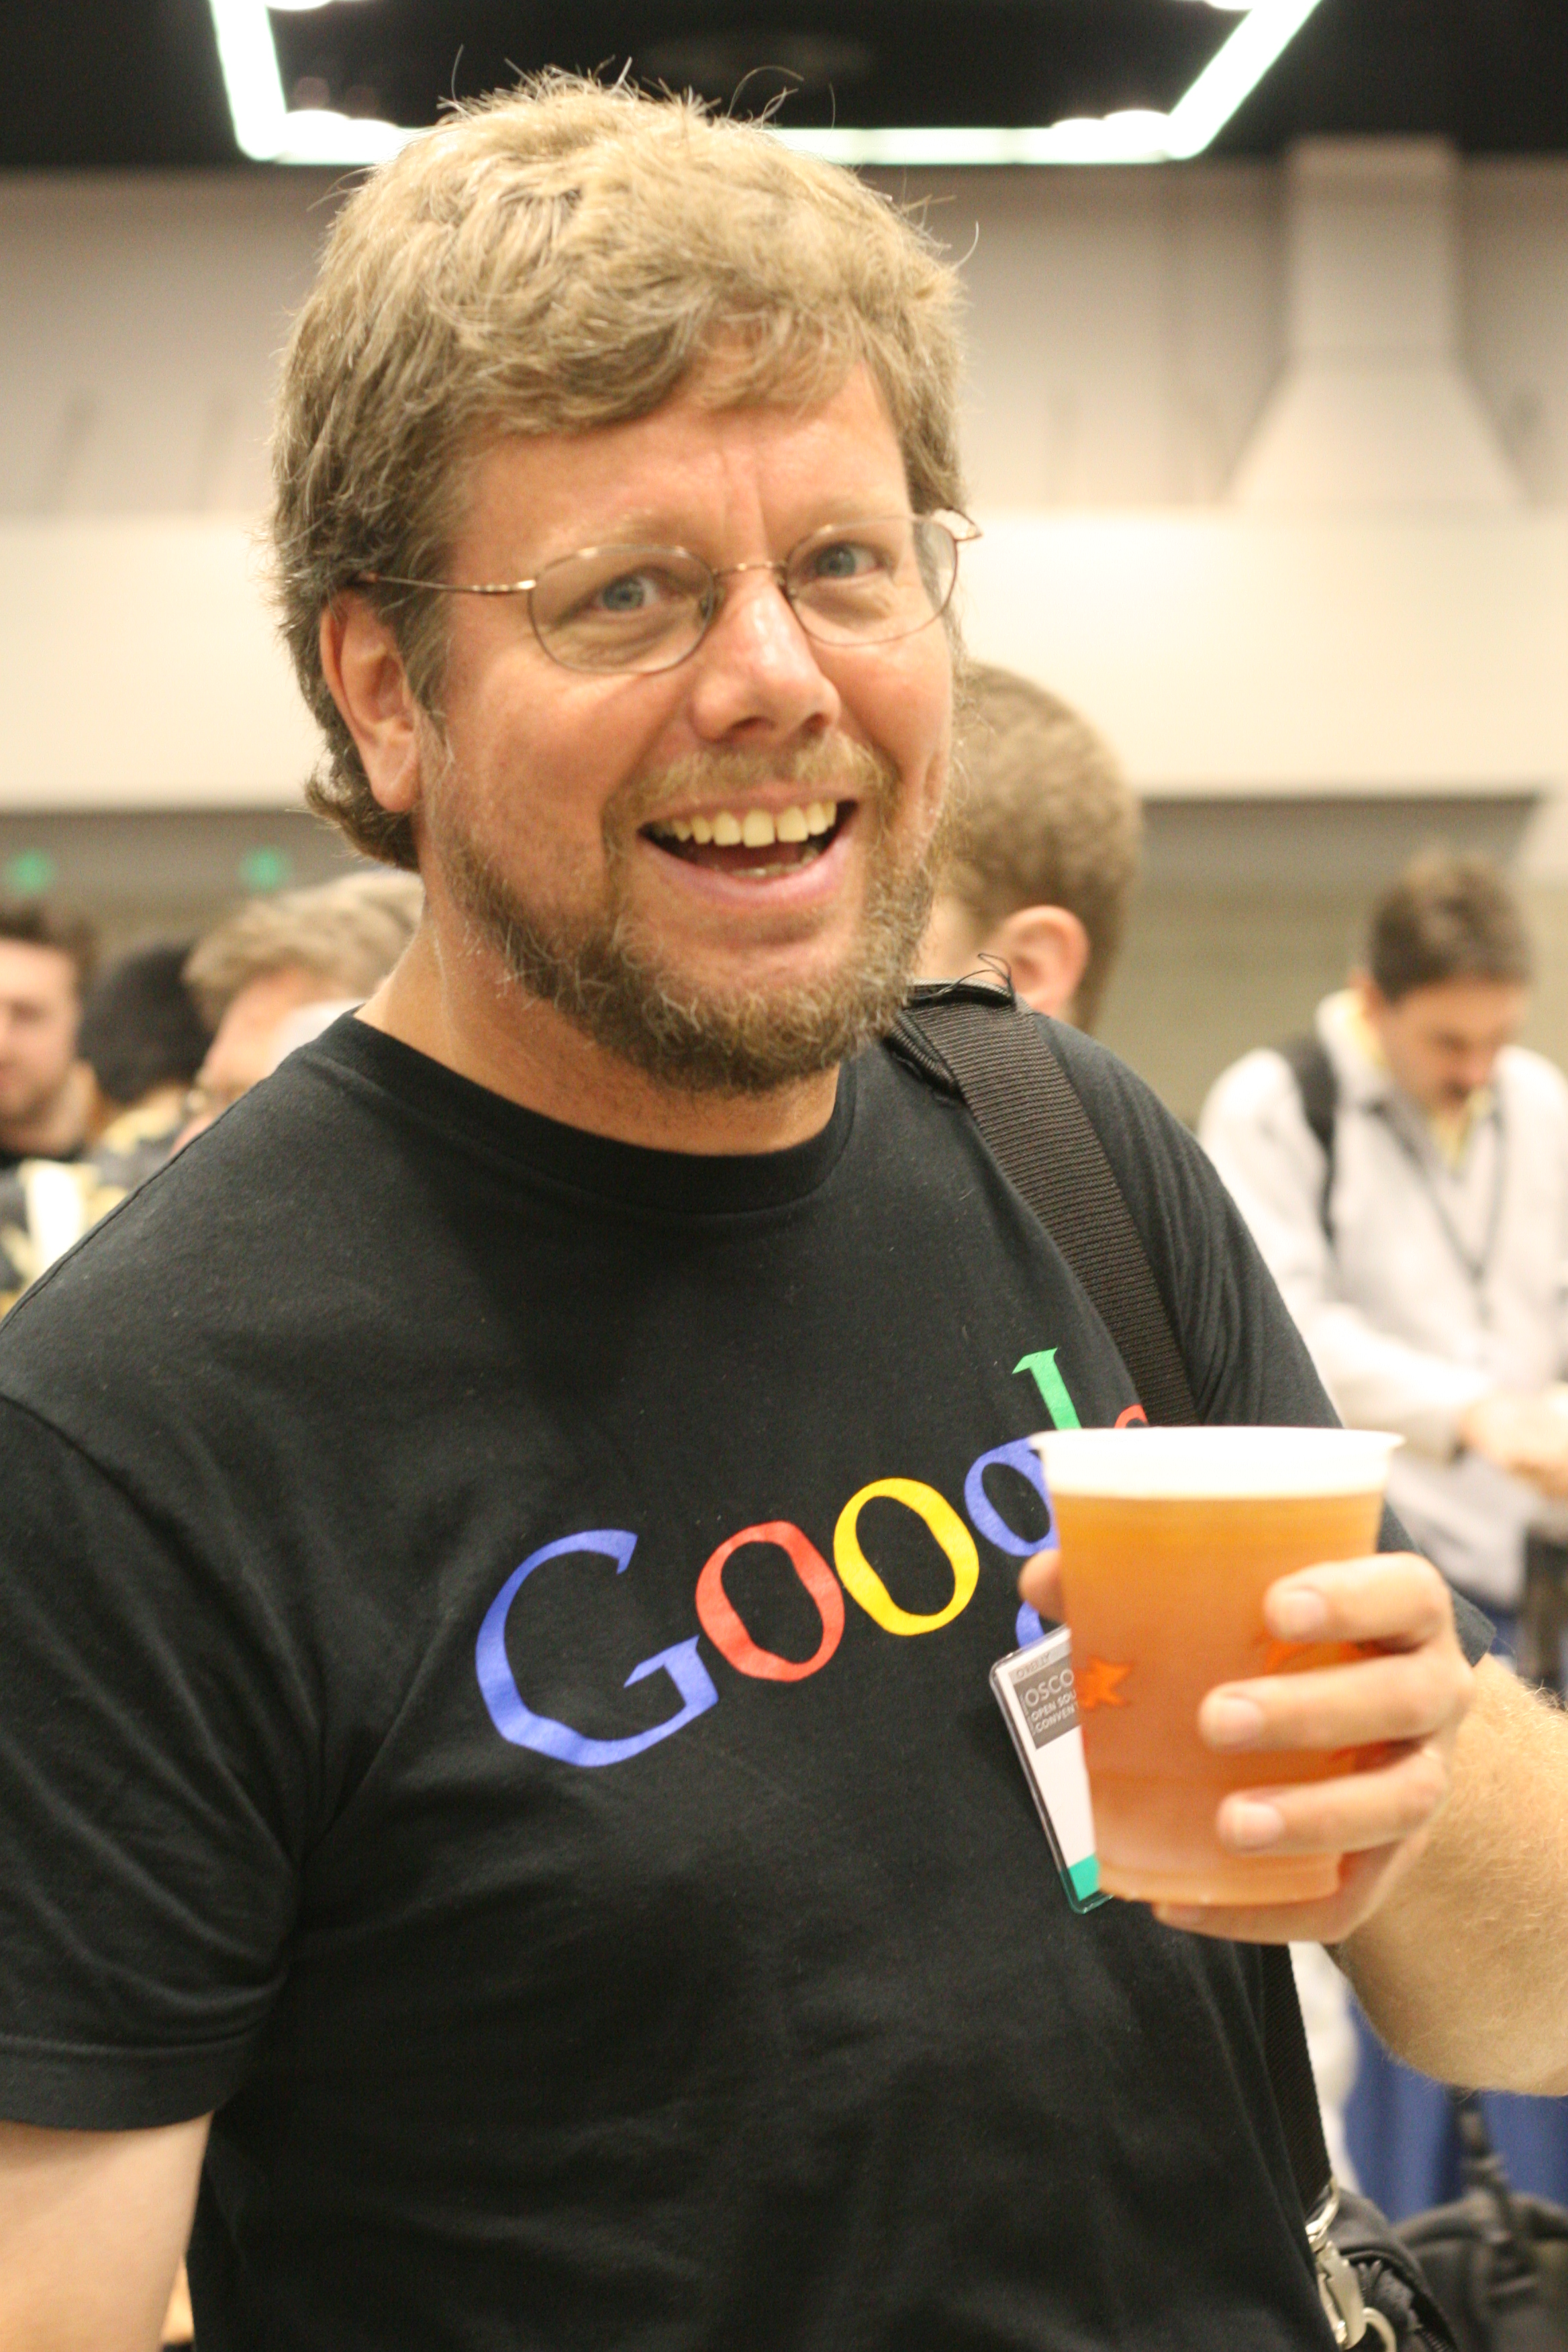
\includegraphics[width=\linewidth]{figs/guido.jpg}
	\end{columns}
\end{frame}

\subsection{Installation}
\begin{frame}{Introduction}{Installation}
\vspace{-0,3cm}
	\begin{itemize}
		\item If you have a good OS such as Linux or Mac, you already have Python!
		\item Otherwise (Windows), you have to install it
			\begin{itemize}
			\item Visit \url{https://www.python.org/downloads/}
			\end{itemize}
		\item Bad news: There is no ``standard'' IDE
			\begin{itemize}
			\item PyCharm, Komodo, PyDev, ...
			\item \url{http://wiki.python.org/moin/PythonEditors}
			\end{itemize}
	\end{itemize}
    \begin{columns}
 	   \column{.40\textwidth}
		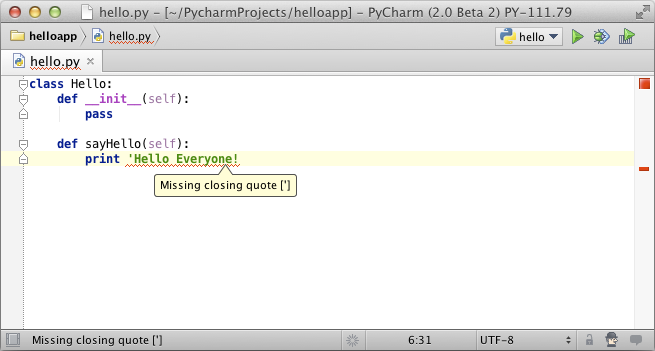
\includegraphics[width=\linewidth]{figs/pycharm.png}\\\centering PyCharm
 	   \column{.35\textwidth}
		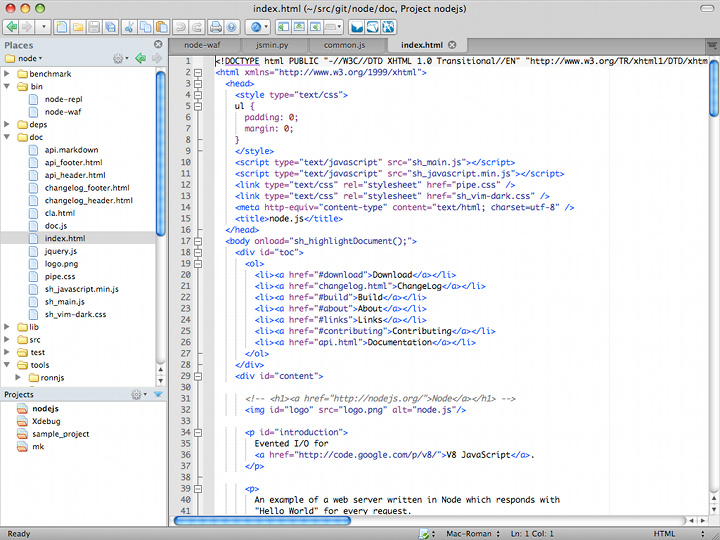
\includegraphics[width=\linewidth]{figs/komodo.png}\\\centering Komodo
 	   \column{.3\textwidth}
		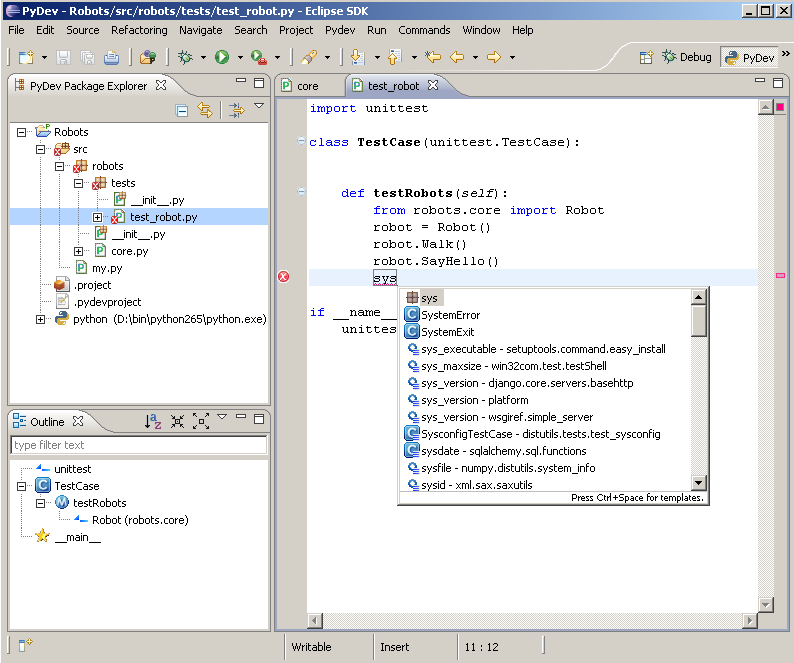
\includegraphics[width=\linewidth]{figs/pydev.png}\\\centering PyDev
	\end{columns}
\end{frame}


\section{The Python interpreter}

\subsection{Python operation modes}
\begin{frame}{The Python interpreter}{Python operation modes}
		Python is an interpreted language, i.e., it needs an interpreter.
			\begin{itemize}
				\item Interpreted = it is not complied = it needs no compilation.
				\item Faster development, slower execution.
			\end{itemize}
		Two operation modes:
			\begin{itemize}
				\item \textbf{Interactive}: The interpreter reads the program from the \textit{stdin} (usually the keyboard).
				\item \textbf{Non-interactive}: The interpreter reads the program from a file (also known as \alert{script}).
			\end{itemize}
\end{frame}

\subsection{Non-interactive}
\begin{frame}[fragile]{The Python interpreter}{Non-interactive}
	The program is in a plain text file.
		\begin{itemize}
		\item It can be edited with any text editor.
		\item Extension ``.py''.
		\item Execution permission (\texttt{chmod u+x myscript.py}).
		\item By default, UTF-8 encoding.
		\end{itemize}
	The first line must be \texttt{\#!/usr/bin/python}
		\begin{itemize}
		\item It is the interpreter location.
		\item If not present, the interpreted must be invoked.
		\end{itemize}

    \begin{columns}
 	   \column{.50\textwidth}
	
		\vspace{-0.2cm}
		\begin{block}{script.py}
		\vspace{-0.2cm}
			\lstinputlisting{code/script.py}
		\end{block}

 	   \column{.50\textwidth}
    	\begin{block}{}
		\begin{verbatim}
		python script.py
		./script.py
		\end{verbatim}
		\end{block}
	\end{columns}
\end{frame}

\subsection{Interactive}
\begin{frame}{The Python interpreter}{Interactive}
		Just run \texttt{python}
			\begin{itemize}
				\item Different names for different versions to avoid conflicts.
				\item \texttt{python}, \texttt{python3.4}, ...
			\end{itemize}

		\vspace{-0.2cm}
		\begin{block}{}
		\vspace{-0.2cm}
			\lstinputlisting[basicstyle=\scriptsize]{code/interprete.txt}
		\end{block}
		The programmer executes as he writes code down.
\end{frame}

\section{An informal introduction}

\subsection{Variables}
\begin{frame}[fragile]{An informal introduction}{Variables (I)}
 	\textbf{Variable}: A name that refers a value.
	\begin{itemize}
		\item No need to declare variables (Python is weakly typed!).
		\item Python automatically assigns types.
		\item Basic types: Numbers, strings and booleans.
	\end{itemize}
	\textbf{Complex data structures}:
		\begin{itemize}
		\item Lists, tuples, dictionaries, associative arrays.
		\end{itemize}

    \begin{columns}
 	   \column{.40\textwidth}
	\begin{block}{Variables}
	\begin{verbatim}
	variable = value
	\end{verbatim}
	\end{block}
	\end{columns}
\end{frame}

\begin{frame}[fragile]{An informal introduction}{Variables (II)}
	\centering \textit{Hint}: \texttt{type()} returns data type.

   	\begin{columns}
   	\column{.50\textwidth}
		\begin{block}{}
		\begin{verbatim}
		>>> integer = 4
		>>> float = 2.3
		>>> integer + float
		6.3
		>>> string = "Spam"
		>>> boolean = True
		>>> a = b = c = 0
		>>> b
		0
		>>> type(integer)
		<type 'int'>
		\end{verbatim}
		\end{block}
	\end{columns}
\end{frame}

\subsection{Numbers}
\begin{frame}[fragile]{An informal introduction}{Numbers (I)}

\vspace{-0.2cm}
	\begin{columns}
 	   			\column{.60\textwidth}
	\textbf{Number types}: Integer, float and complex.

 	   			\column{.40\textwidth}
				\begin{block}{}
				\begin{verbatim}
				>>> num = 1+3j
				>>> num
				(1+3j)
				\end{verbatim}
				\end{block}
		\end{columns}

    \vspace{-0.2cm}
    %\begin{columns}
    %\column{.30\textwidth}
	\begin{center}
	\bigskip
		\centering \begin{tabular}{cl|cl}\hline
		\sc Sign & \sc Operator 	& \sc Sign 	& \sc Operator \\ \hline
		= 	 & Assignment   & // 	& Floor division\footnote{Only Python 3.x}\\
		+ 	& Add  			& **	& Exponent \\
		- 	& Substration 	& +=	& Assign + \\
		* 	& Multiplication& -=	& Assign - \\
		/ 	& Division 		& *=	& Assign * \\
		\% 	& Modulus 		& /=	& Assign /\\\hline
		\end{tabular}
	\end{center}
	%\end{columns}
\end{frame}

\begin{frame}[fragile]{An informal introduction}{Numbers (II)}
    %\vspace{-0.2cm}
    \begin{columns}
    \column{.60\textwidth}
		\begin{block}{ArithmeticDemo.py}
		\lstinputlisting{code/operdemo.py}
		\end{block}
	\end{columns}

	\bigskip
    New Python elements:
    \begin{itemize}
        \item The \texttt{input()} function.
		\item The \texttt{int()} and \texttt{float()} functions.
    \end{itemize}
\end{frame}
\subsection{Strings}
\begin{frame}[fragile]{An informal introduction}{Strings (I)}
   	\begin{columns}
    	\column{.30\textwidth}
		\begin{block}{}
		\begin{verbatim}
		>>> 'hello'
		'hello'
		>>> "hello"
		'hello'
		\end{verbatim}
		\end{block}

    	\column{.70\textwidth}
		Strings are delimited with single or double quotes, they can be used together.
	\end{columns}

   	\begin{columns}
    			\column{.30\textwidth}
			Triple quotes to define multi-line strings.

    			\column{.70\textwidth}
		\begin{block}{}
			\begin{verbatim}
			>>> """hello
			... there are multiple lines"""
			'hello\nthere are multiple lines'
			\end{verbatim}
			\end{block}
	\end{columns}
	\bigskip
	As C, C++ or Java, `\textbackslash n' means carriage return.
\end{frame}

\begin{frame}[fragile]{An informal introduction}{Strings (II)}
	Of course, variables can contain strings.
	\begin{block}{}
		\begin{verbatim}
		>>> text = "hello"
		>>> print(text)
		hello
		\end{verbatim}
	\end{block}

    New Python elements:
    \begin{itemize}
        \item The \texttt{print()} function.
    \end{itemize}
\end{frame}




\begin{frame}[fragile]{An informal introduction}{Strings (III)}
\vspace{-0.4cm}
	\begin{columns}
 	   			\column{.40\textwidth}
		Strings contatenation
				\begin{block}{}
				\begin{verbatim}
				>>> "hello" + " there"
				'hello there'
				>>> "hello" "there"
				'hellothere'
				\end{verbatim}
				\end{block}

 	   			\column{.30\textwidth}
		Variables with strings
				\begin{block}{}
				\begin{verbatim}
				>>> a = "hello"
				>>> b = " there"
				>>> a + b
				'hello there'
				\end{verbatim}
				\end{block}

 	   			\column{.30\textwidth}
		String length
				\begin{block}{}
				\begin{verbatim}
				>>> len("hello")
				5
				\end{verbatim}
				\end{block}
		\end{columns}

\end{frame}

\begin{frame}[fragile]{An informal introduction}{Strings (IV)}
	\vspace{-0.2cm}
	Strings can be used as a sequence of characters: \textit{Slice notation}.
	\begin{itemize}
	\item Quite common in Python data structures.
	\item It uses indices (as an array). First index is $0$.
	\end{itemize}
	\vspace{-0.3cm}
	\begin{columns}
 	   			\column{.40\textwidth}
				\begin{block}{}
				\begin{verbatim}
				>>> a = "hello"
				>>> a[2]
				'l'
				>>> a[2:]
				'llo'
				>>> a[:2]
				'he'
				>>> a[2:] + a[:2]
				'llohe'
				>>> a[2:4]
				'll'
				\end{verbatim}
				\end{block}
		\end{columns}
\end{frame}

\subsection{Lists}
\begin{frame}[fragile]{An informal introduction}{Lists (I)}
	\textbf{List}: An ordered collection of mutable data.
	\begin{itemize}
		\item Very powerful data structure, similar to an array.
		\item \textit{Ordered}: Data in the list have a location.
		\item \textit{Mutable}: Data can be modified.
		\item Data types can be different.
	\end{itemize}
	\begin{columns}
   		\column{.70\textwidth}
		\begin{block}{List initialization}
		\begin{verbatim}
		variable = [data1, data2, ..., dataN]
		\end{verbatim}
		\end{block}
	\end{columns}
\end{frame}

\begin{frame}[fragile]{An informal introduction}{Lists (II)}
	\begin{columns}
 	   	\column{.40\textwidth}
		Definition example

   		\column{.60\textwidth}
		\begin{block}{}
		\begin{verbatim}
		>>> a = ['spam', 'eggs', 123]
		>>> a
		['spam', 'eggs', 123]
		\end{verbatim}
		\end{block}
	\end{columns}

	\begin{columns}
 	   	\column{.40\textwidth}
		Slice notation and the \texttt{len()} function work on lists

   		\column{.60\textwidth}
		\begin{block}{}
		\begin{verbatim}
		>>> a[2]
		123
		>>> a[1:]
		['eggs', 123]
		>>> a + a[2:len(a)]
		['spam', 'eggs', 123, 123]
		\end{verbatim}
		\end{block}
	\end{columns}
\end{frame}

\section{Control flow}
\subsection{Conditions}

\begin{frame}[fragile]{Control flow}{Conditions (I)}
	Conditional statements implement decision making
	\begin{itemize}
	\item Decide some code has to be executed or not.
	\item The result is a boolean.
	\item Execute code if condition is satisfied.
	\end{itemize}

	\begin{columns}
 	   	\column{.40\textwidth}
	\begin{block}{\texttt{if} statement}
		\begin{verbatim}
		if condition:
		    # Some code
		else:
		    # Some other code
		\end{verbatim}
		\end{block}
	\end{columns}

   New Python elements:
	\begin{itemize}
	\item Comments begin with '\#'.
	\item \alert{Indentation plays a mayor role: It defines code bodies.}
	\end{itemize}
	
\end{frame}

\begin{frame}[fragile]{Control flow}{Conditions (II)}
	\begin{block}{Condition example}
	\vspace{-0.2cm}
		\lstinputlisting[basicstyle=\scriptsize]{code/if.py}
	\end{block}
	\tiny{\href{http://anh.cs.luc.edu/python/hands-on/3.1/handsonHtml/ifstatements.html}{(Source)}}
	\\
	\normalsize{
	New Python element:
		\begin{itemize}
		\item Comparison operators.
		\end{itemize}
	}
\end{frame}

\begin{frame}[fragile]{Control flow}{Conditions (III)}
	\centering \begin{tabular}{cl|cl}\hline
	\sc Sign & \sc Operator & \sc Sign 	& \sc Operator \\ \hline
	== 	 & Equal   		& \texttt{and} 	& Logical and \\
	!= 	& Not equal  	& \texttt{or}	& Logical or  \\
	> 	& Greater 		& \texttt{not}	& Logical not \\
	< 	& Lower			&   	& \\
	>= 	& Greater or equal 		& 	& \\
	<= 	& Lower or equal 		& 	& \\\hline
	\end{tabular}

	\bigskip

	Example: \texttt{((age > 18) or (name == 'Biggus Dickus'))}
\end{frame}

\subsection{While loop}
\begin{frame}{Control flow}{While loop}
	\begin{block}{Fibonacci series}
	\vspace{-0.2cm}
		\lstinputlisting[basicstyle=\scriptsize]{code/fibo.py}
	\end{block}

    New Python elements:
	\begin{itemize}
	\item Multiple assignments.
	\end{itemize}
	
\end{frame}

\section{Examples}
\subsection{Example 1: Multiplication table}
\begin{frame}{Examples}{Example 1: Multiplication table}
	\begin{block}{multi.py}
		\lstinputlisting[basicstyle=\scriptsize]{code/multi.py}
	\end{block}
		\tiny{\href{http://www.pythonforbeginners.com/basics/using-math-in-python/}{Source}}
\end{frame}

\IfStrEq{\modo}{ASC}{
	\begin{frame}[plain]{Practice}{Numbers}
		\begin{enumerate}
		\item Given the second-grade equation $a x^2 + b x + c = 0$, write a program that asks for coefficients $a$, $b$ and $c$, and then computes the value of $x$ with the following equation
		\begin{equation*}
		x = \frac{-b \pm \sqrt{b^2 - 4 a c}}{2a}
		\end{equation*}
		\end{enumerate}
	\end{frame}
	}{}

\appendix
\section<Bibliographic references>*{\appendixname}
\subsection<Bibliographic references>*{Bibliographic references}

\begin{frame}[plain,allowframebreaks]
  \frametitle<presentation>{Bibliographic references}

  \begin{thebibliography}{4}

  \beamertemplatebookbibitems
  % libro
   \bibitem{vanRosum}[van Rosum, 2012]
    G. van Rossum, Jr. Fred L. Drake.
    \newblock \emph{Python Tutorial Release 3.2.3, chapters 2 and 3}.
    \newblock Python Software Foundation, 2012. 
  % libro
     \bibitem{Bahit}[Bahit, 2008]
     E. Bahit.
    \newblock \emph{Curso: Python para principiantes}.
    \newblock Creative Commons Atribución-NoComercial 3.0, 2012.
    
  % libro
    \bibitem{Swaroop}[Swaroop, 2008]
     C H.  Swaroop.
    \newblock \emph{A Byte of Python}.
    \newblock Creative Commons Attribution-ShareAlike 3.0, 2008.

  \bibitem{Pilgrim}[Pilgrim, 2004]
  M. Pilgrim.
    \newblock \emph{Dive into Python}.
    \newblock Ed. Prentice Hall, 2004.
   
    
 
  \end{thebibliography}
\end{frame}



\end{document}
